\section{Benchmark details}
Next, we have a closer look at some of the benchmarks and see how the effectiveness of each optimisation depends on the characteristics of the source code. The first section of Table \ref{tbl-performance-per-benchmark} shows the distribution of the JVM instructions executed in each benchmark, and both the maximum and average number of bytes on the JVM stack. We can see some important differences between the benchmarks. While the sort benchmarks on the left are almost completely load/store bounded, XXTEA, RC5 and MD5 are much more computation intensive, spending fewer instructions on loads and stores, and more on math or bitwise operations. The left three benchmarks and the outlier detection benchmark have only a few bytes on the stack, but as the benchmarks contain more complex expressions, the number of values on the stack increases.

The second part of tables \ref{tbl-performance-per-benchmark} and \ref{tbl-codesize-per-benchmark} first shows the overhead before optimisation, split up in the five instruction categories. We then list the effect of each optimisation on the total overhead. Finally we show the overhead per category after applying all optimisations.

The improved peephole optimiser and stack caching both target the push/pop overhead. Stack caching can eliminate almost all, and replaces the need for a peephole optimiser, but it is interesting to compare the two. The improved peephole optimiser does well for the simple benchmarks like sort, binary search and outlier detection, leaving less overhead to remove for stack caching. The more computation intensive benchmarks contain more complicated expressions, which means there is more distance between a push and a pop, leaving more cases that cannot be handled by the peephole optimiser. For these benchmarks, replacing the peephole optimiser with stack caching yields a big improvement.

The benchmarks on the left spend more time on load/store instructions. This results in higher load/store overhead, and the two optimisations that target this overhead, popped value caching and mark loops, have a big impact. For the computation intensive benchmarks, the load/store overhead is much smaller, but the higher stack size means stack caching is very important for these benchmarks.

The smaller benchmarks highlight certain specific aspects of our approach, while the larger CoreMark benchmark covers a mix of different types of processing. As a result, it is an average case in almost every row in Table \ref{tbl-performance-per-benchmark}. The reason it ends up being the third slowest after all optimisations was discussed in \ref{sec-evaluation-coremark-unfair-optimisations}. With the 'unfair' optimisations described there, CoreMark's performance overhead would be 61\%, very close to the average of the other benchmarks.

\subsubsection{Bubble sort}
\label{sec-evaluation-bubble-sort}
Next we look at bubble sort in some more detail. After optimisation, we see most of the stack related overhead has been eliminated and of the 101.2\% remaining performance overhead, most is due to other sources. For bubble sort there is a single, clearly identifiable source. When we examine the detailed trace output,  79.8\% is due to \mycode{ADD} instructions, but bubble sort hardly does any additions. This is a good example of how the simple JVM instruction set leads to less efficient code. To access an array we need to calculate the address of the indexed value, which takes one move and five additions for an array of shorts. This calculation is repeated for each access, while the C version has a much more efficient approach, using the auto-increment version of the AVR's LD and ST instructions to slide a pointer over the array. Of the remaining 101.2\% overhead, 93.1\% is caused by these address calculations.
% ADD, ADC and ADIW all cost 26.6\%. Each array access does 1 MOVW, 2 ADDs, 2 ADCs and 1 ADIW.
% 26.6*3+26.6/2 = 93.1

%\paragraph{Bit shifts} Interestingly, the reason fft is the slowest, is similar to the reason rc5 is fastest: they both spend a large amount of time doing bit shifts. Rc5 shifts by a variable, but large number of bits. Only 8.0\% of the executed JVM instructions are bit shifts, but they account for 71\% of the execution time in the optimised version. For these variable bit shifts, our translator and \mycode{avr-gcc} generate a similar loop, so the two share a large constant factor.
%
%On the other hand fft is a hard case because it does many constant shifts by exactly 6 bits. For these, our VM simply emits 6 single shifts, which is slower than the special case \mycode{avr-gcc} emits for shifts by exactly 6 bits.  While we could do the same, we feel this special case is too specific to include in our VM.

\subsubsection{HeatCalib}
Looking at the code size data in Table \ref{tbl-codesize-per-benchmark}, we see the HeatCalib benchmark has a negative code size overhead. This is caused by the fact that we compile the C versions using \mycode{avr-gcc}'s -O3 optimisations, optimising for performance instead of code size. In this case, as well as for FFT, this caused \mycode{avr-gcc} to duplicate a part of code, which improves performance but at the cost of a significantly larger code size.

\subsubsection{MoteTrack}
The MoteTrack benchmark is by far the slowest of our benchmarks, at a 165\% overhead compared to native C. MoteTrack stores a database of reference signatures in Flash. In C this is a complex struct containing a number of sub-structures and fixed-sized arrays, while it becomes a collection of objects and arrays in Java, shown in \ref{fig-motetrack-refsignature-objects}.

Since the layout of the complete C structure is known at compile time, the C function to load a reference signature from its database can simply use \mycode{memcpy\_P} to copy a block of 80 bytes from Flash to RAM. For Java, the method to read from Flash must follow multiple pointers to follow several indirections to find the locations to put each value. As a result, reading a single signature takes 1695 cycles in Java, and only 735 cycles in C.
% 68.5% overhead from reading refSignatures from Flash. 68.5 / 1695 * 735 = 29.7

\subsubsection{LEC}
In Section \ref{sec-introduction-performance} we calculated that, the LEC compression algorithm, reduced the energy spent to transmit our sample ECG data by 650 μJ, at the expense of 246 μJ spent on CPU cycles compressing the data, when implemented in C and using the ATmega128 CPU and CC2420 radio.

A compression algorithm like LEC is a good example of an optimisation that may be part of an application loaded onto a sensor node. However, if the overhead of using a VM is too high, the cost of compression may outweight the energy saved on transmission. Table \ref{tbl-performance-per-benchmark} shows that using the baseline AOT approach, the LEC benchmark has an overhead of 278.4\%. Because the CPU has to stay active longer, this means compressing the data would cost $246 \mu J * 3.784 = 930 \mu J$, which is more than the 650 μJ saved on transmission.

After we apply our optimisations, the overhead is reduced to 86.5\%, resulting in $246 \mu J * 1.685 = 459 \mu J$ spent on compression. While the savings are less than when we use native C to compress the data, our optimisations mean we can save on transmission costs by using LEC compression, while using the baseline AOT approach, LEC compression would have resulted in a net loss.

\subsubsection{Xxtea and the mark loops optimisation}

\begin{figure}
\centering
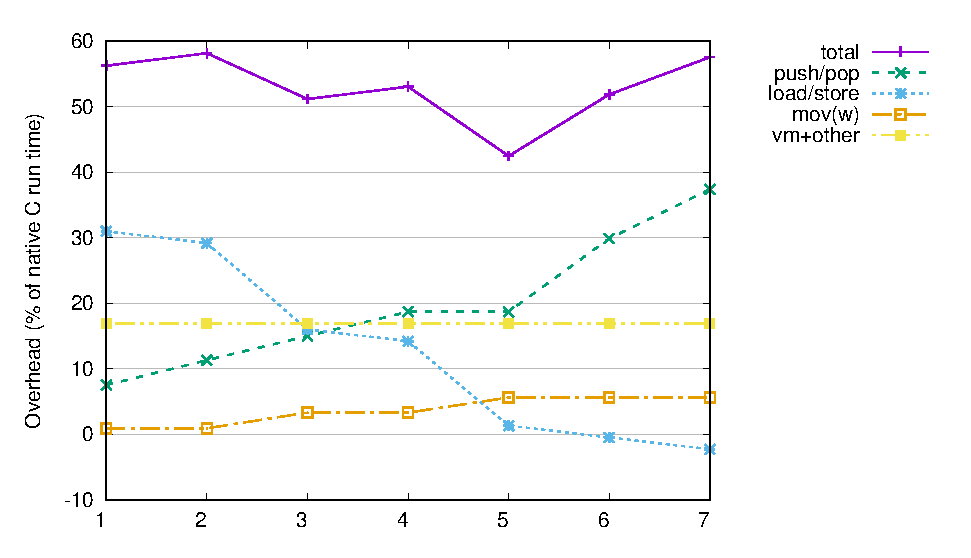
\includegraphics[width=\mygraphsize]{pinnedregs-performance-xxtea.eps}
\caption{Xxtea performance overhead for different number of pinned register pairs}
\label{fig-performance-pinnedregs-xxtea-per-opcode-category}
\end{figure}

\begin{figure}
\centering
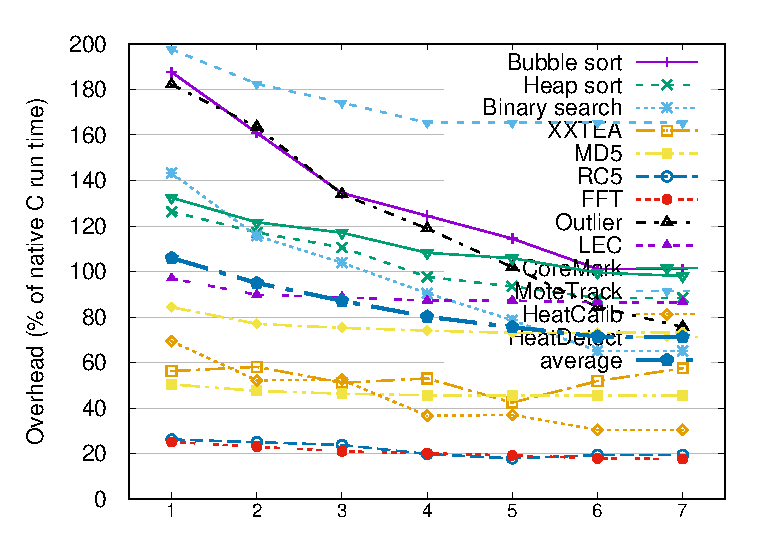
\includegraphics[width=\mygraphsize]{pinnedregs-performance-all-benchmarks.eps}
\caption{Per benchmark performance overhead different number of pinned register pairs}
\label{fig-performance-pinnedregs-per-benchmark}
\end{figure}

Perhaps the most interesting benchmark is xxtea. Its high average stack depth means popped value caching does not have much effect: most registers are used for real stack values, leaving few chances to reuse a value that was previously popped from the stack. 

When we apply the mark loops optimisation, performance actually degrades by 5\%, and code size overhead increases 6\%! Here we have an interesting tradeoff: if we use a register to pin a variable, accessing that variable will be cheaper, but this register will no longer be available for stack caching, so more stack values may have to be spilled to memory.

For most benchmarks the maximum of 7 register pairs to pin variables to was also the best option. At a lower average stack depth, the fewer number of registers available for stack caching is easily compensated for by the cheaper variable access. For xxtea however, the cost of spilling more stack values to memory outweighs the gains of pinning more variables when too many variables are pinned. Figure \ref{fig-performance-pinnedregs-xxtea-per-opcode-category} shows the overhead for xxtea from the different instruction categories. When we increase the number of register pairs used to pin variables from 1 to 7, the load/store overhead steadily decreases, but the push/pop and move overhead increase. For XXTEA, the optimum is at 5 pinned register pairs, at which the total overhead is only 43\%, instead of 58\% at 7 pinned register pairs.

Interestingly, when we pin 7 pairs, the AOT version actually does fewer loads and stores than the C compiler. Under high register pressure the C version may spill a register value to memory and later load it again, adding extra load/store instructions. When the AOT version pins too many registers, it will also need to spill values, but this adds push/pop instructions instead of loads/stores.

Figure \ref{fig-performance-pinnedregs-per-benchmark} shows the performance for each benchmark, as the number of pinned register pairs is increased. The benchmarks stay stable or even slow down when the number pinned pairs is increased beyond 5 are the benchmarks that have a high stack depth, while the benchmarks with low stack depth such as sort, search and outlier detection improve significantly. It should be possible to develop a simple heuristic to allow the VM to make a better decision on the number of registers to pin. Since our current VM always pins 7 pairs, we used this as our end result and leave this heuristic to future work.

